\documentclass[a4paper, fontsize=12pt]{article}
\input ../../my_simple_preamble.tex
\usepackage{pgfplots}
\pgfplotsset{compat=1.15}
\usepackage{mathrsfs}
\usepackage{mathtools}
\usetikzlibrary{arrows}

\begin{titlepage}
    \title{Контрольная работа №2}
    \author{Морозов Н.Ю. 23.Б09}
    \date{}
\end{titlepage}

\begin{document}
    \maketitle

    \section{}

    Морозов - [14, 16, 18, 16, 9, 16, 3]

    \begin{figure}[ht]
        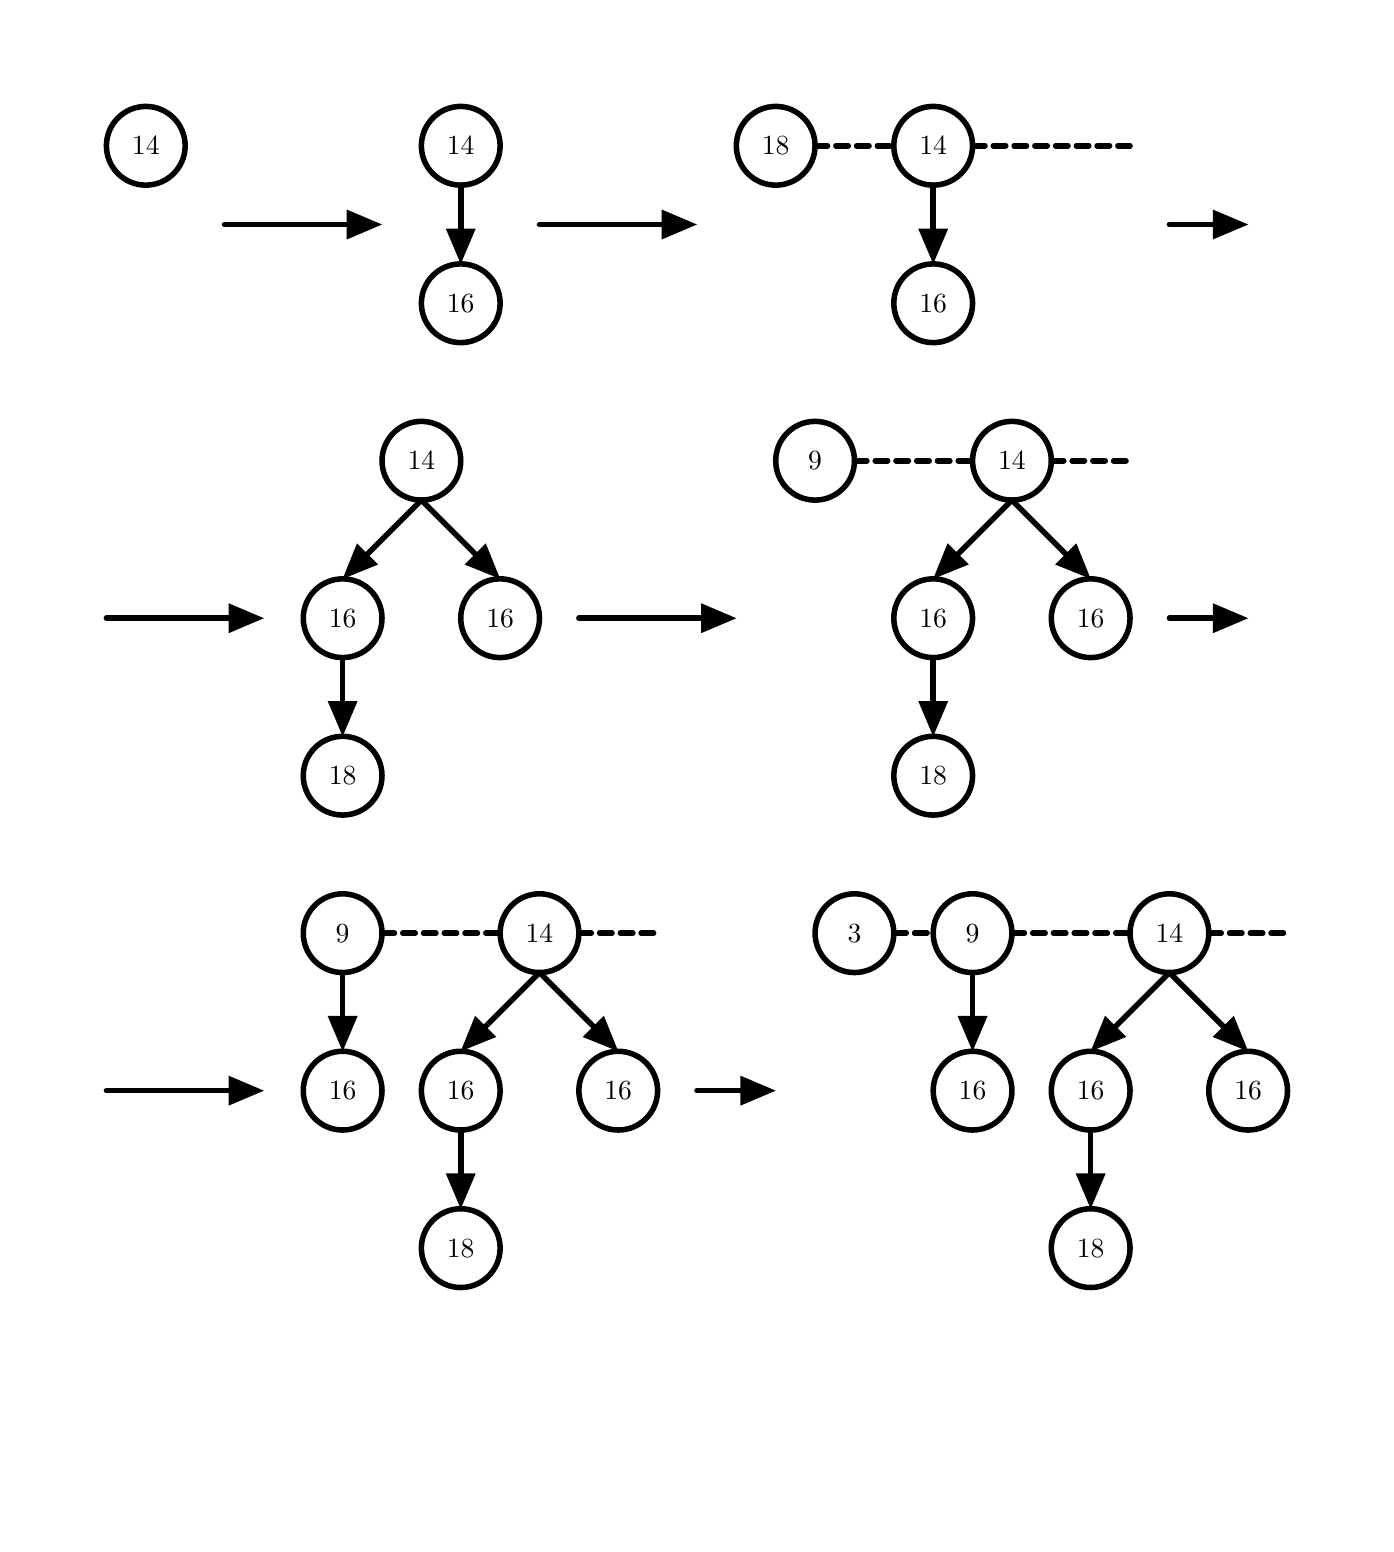
\begin{tikzpicture}[line cap=round,line join=round,>=triangle 45,x=1.0cm,y=1.0cm]
            \clip(0.,-7.) rectangle (17.,12.);

            \draw [line width=2.pt] (1.5,10.5) circle (0.5cm) node {$14$};

            \draw [->,line width=2.pt] (2.5,9.5) -- (4.5,9.5);
            \draw [line width=2.pt] (5.5,10.5) circle (0.5cm) node {$14$};
            \draw [->,line width=2.pt] (5.5,10.) -- (5.5,9.);
            \draw [line width=2.pt] (5.5,8.5) circle (0.5cm) node {$16$};

            \draw [->,line width=2.pt] (6.5,9.5) -- (8.5,9.5);
            \draw [line width=2.pt] (9.5, 10.5) circle (0.5cm) node {$18$};
            \draw [line width=2.pt, dash pattern=on  4.5pt off 3pt] (10., 10.5) -- (11., 10.5);
            \draw [line width=2.pt] (11.5,10.5) circle (0.5cm) node {$14$};
            \draw [->,line width=2.pt] (11.5,10.) -- (11.5,9.);
            \draw [line width=2.pt] (11.5,8.5) circle (0.5cm) node {$16$};
            \draw [line width=2.pt, dash pattern=on  4.5pt off 3pt] (12.,10.5) -- (14.,10.5);
            \draw [->,line width=2.pt] (14.5,9.5) -- (15.5,9.5);


            \draw [->,line width=2.pt] (1.0,4.5) -- (3.0,4.5);
            \draw [line width=2.pt] (5.0,6.5) circle (0.5cm) node {$14$};
            \draw [->, line width=2.pt] (5.0,6.) -- (4.,5.);
            \draw [->, line width=2.pt] (5.,6.) -- (6.,5.);
            \draw [line width=2.pt] (4.,4.5) circle (0.5cm) node {$16$};
            \draw [line width=2.pt] (6.,4.5) circle (0.5cm) node {$16$};
            \draw [->, line width=2.pt] (4.,4.) -- (4.,3.);
            \draw [line width=2.pt] (4.,2.5) circle (0.5cm) node {$18$};
            \draw [->,line width=2.pt] (7,4.5) -- (9,4.5);

            \draw [line width=2.pt] (10.,6.5) circle (0.5cm) node {$9$};
            \draw [line width=2.pt, dash pattern=on  4.5pt off 3pt] (10.5,6.5) -- (12.,6.5);
            \draw [line width=2.pt] (12.5,6.5) circle (0.5cm) node {$14$};
            \draw [line width=2.pt, dash pattern=on  4.5pt off 3pt] (13,6.5) -- (14.,6.5);
            \draw [->, line width=2.pt] (12.5,6.) -- (11.5,5.);
            \draw [->, line width=2.pt] (12.5,6.) -- (13.5,5.);
            \draw [line width=2.pt] (11.5,4.5) circle (0.5cm) node {$16$};
            \draw [line width=2.pt] (13.5,4.5) circle (0.5cm) node {$16$};
            \draw [->, line width=2.pt] (11.5,4.) -- (11.5,3.);
            \draw [line width=2.pt] (11.5,2.5) circle (0.5cm) node {$18$};
            \draw [->,line width=2.pt] (14.5,4.5) -- (15.5,4.5);


            \draw [->,line width=2.pt] (1.0,-1.5) -- (3.0,-1.5);
            \draw [line width=2.pt] (4.,0.5) circle (0.5cm) node {$9$};
            \draw [->, line width=2.pt] (4.,0.) -- (4.,-1.);
            \draw [line width=2.pt] (4.,-1.5) circle (0.5cm) node {$16$};
            \draw [line width=2.pt, dash pattern=on  4.5pt off 3pt] (4.5,0.5) -- (6.,0.5);
            \draw [line width=2.pt] (6.5,0.5) circle (0.5cm) node {$14$};
            \draw [line width=2.pt, dash pattern=on  4.5pt off 3pt] (7.,0.5) -- (8.,0.5);
            \draw [->, line width=2.pt] (6.5,0.) -- (5.5,-1.);
            \draw [->, line width=2.pt] (6.5,0.) -- (7.5,-1.);
            \draw [line width=2.pt] (5.5,-1.5) circle (0.5cm) node {$16$};
            \draw [line width=2.pt] (7.5,-1.5) circle (0.5cm) node {$16$};
            \draw [->, line width=2.pt] (5.5,-2.) -- (5.5,-3.);
            \draw [line width=2.pt] (5.5,-3.5) circle (0.5cm) node {$18$};
            
            \draw [->,line width=2.pt] (8.5,-1.5) -- (9.5,-1.5);
            \draw [line width=2.pt] (10.5,0.5) circle (0.5cm) node {$3$};
            \draw [line width=2.pt, dash pattern=on  4.5pt off 3pt] (11.,0.5) -- (11.5,0.5);
            \draw [line width=2.pt] (12.0,0.5) circle (0.5cm) node {$9$};
            \draw [->, line width=2.pt] (12.0,0.) -- (12.0,-1.);
            \draw [line width=2.pt] (12.0,-1.5) circle (0.5cm) node {$16$};
            \draw [line width=2.pt, dash pattern=on  4.5pt off 3pt] (12.5,0.5) -- (14.,0.5);
            \draw [line width=2.pt] (14.5,0.5) circle (0.5cm) node {$14$};
            \draw [line width=2.pt, dash pattern=on  4.5pt off 3pt] (15.,0.5) -- (16.,0.5);
            \draw [->, line width=2.pt] (14.5,0.) -- (13.5,-1.);
            \draw [->, line width=2.pt] (14.5,0.) -- (15.5,-1.);
            \draw [line width=2.pt] (13.5,-1.5) circle (0.5cm) node {$16$};
            \draw [line width=2.pt] (15.5,-1.5) circle (0.5cm) node {$16$};
            \draw [->, line width=2.pt] (13.5,-2.) -- (13.5,-3.);
            \draw [line width=2.pt] (13.5,-3.5) circle (0.5cm) node {$18$};                
            \end{tikzpicture}
    \end{figure}

\section{}

МОРОЗОВНИКИТАЮРЬЕВИЧ

\noindent $ _0\text{М}_0\text{O}_0\text{Р}_2\text{З}_2\text{В}_0\text{Н}_0\text{И}_0\text{К}_7
\text{Т}_0\text{А}_0\text{Ю}_3\text{Ь}_0\text{Е}_0\text{В}_7\text{Ч}0\$$

\noindent $\underbracket{\text{\ М}}\ \underbracket{\text{О}}\ \underbracket{\text{Р}}\ 
\underbracket{\text{ОЗ}}\ \underbracket{\text{ОВ}}\ \underbracket{\text{Н}}\ \underbracket{\text{И}}\ 
\underbracket{\text{К}}\ \underbracket{\text{ИТ}}\ \underbracket{\text{А}}\ \underbracket{\text{Ю}}\ 
\underbracket{\text{РЬ}}\ \underbracket{\text{Е}}\ \underbracket{\text{В}}\ \underbracket{\text{ИЧ} }\ 
\underbracket{ \text{\$}}$

\section{}

\begin{figure}[ht]
    \begin{tikzpicture}[line cap=round,line join=round,>=triangle 45,x=1.0cm,y=1.0cm]
        \clip(0.,0.) rectangle (18.,18.);
        
        \draw [line width=2.pt] (1,9)-- (10.,1.) node[midway,sloped,above] {РОЗОВНИК\$};
        \draw [line width=2.pt] (1,9)-- (10.,3.) node[midway,sloped,above] {O\$};
        \draw [line width=2.pt] (1,9)-- (10.,5.) node[midway,sloped,above] {НИК\$};
        \draw [line width=2.pt] (1,9)-- (10.,7.) node[midway,sloped,above] {МОРОЗОВНИК\$};
        \draw [line width=2.pt] (1,9)-- (10, 9) node[midway,sloped,above] {К\$};
        \draw [line width=2.pt] (1,9)-- (10,11) node[midway,sloped,above] {ИК\$};
        \draw [line width=2.pt] (1,9)-- (10,13) node[midway,sloped,above] {ЗОВНИК\$};
        \draw [line width=2.pt] (1,9)-- (10,15) node[midway,sloped,above] {ВНИК\$};
        \draw [line width=2.pt] (1,9)-- (10,17) node[midway,sloped,above] {\$};
        \draw [line width=2.pt] (10.,3.)-- (15.,3.) node[midway,sloped,above] {ВНИК\$};
        \draw [line width=2.pt] (10.,3.)-- (15.,1.) node[midway,sloped,above] {ЗОВНИК\$};
        \draw [line width=2.pt] (10.,3.)-- (15.,5.) node[midway,sloped,above] {РОЗОВНИК\$};

        \fill [fill=white, draw=black, line width=2.pt] (1.,9.) circle (0.5cm) node {$1$};
        \fill [fill=white, draw=black, line width=2.pt] (10.,1.) circle (0.5cm) node {$3$};
        \fill [fill=white, draw=black, line width=2.pt] (10.,3.) circle (0.5cm) node {$4$};
        \fill [fill=white, draw=black, line width=2.pt] (10.,5.) circle (0.5cm) node {$9$};
        \fill [fill=white, draw=black, line width=2.pt] (10.,7.) circle (0.5cm) node {$1$};
        \fill [fill=white, draw=black, line width=2.pt] (10.,9.) circle (0.5cm) node {$11$};
        \fill [fill=white, draw=black, line width=2.pt] (10,11) circle (0.5cm) node {$10$};
        \fill [fill=white, draw=black, line width=2.pt] (10,13) circle (0.5cm) node {$6$};
        \fill [fill=white, draw=black, line width=2.pt] (10.,15) circle (0.5cm) node {$8$};
        \fill [fill=white, draw=black, line width=2.pt] (10,17) circle (0.5cm) node {$12$};
        \fill [fill=white, draw=black, line width=2.pt] (15.,1.) circle (0.5cm) node {$7$};
        \fill [fill=white, draw=black, line width=2.pt] (15.,3.) circle (0.5cm) node {$5$};
        \fill [fill=white, draw=black, line width=2.pt] (15.,5.) circle (0.5cm) node {$9$};
        \end{tikzpicture}
\end{figure}

\end{document}